\documentclass[11pt,a4paper]{article}
\usepackage[margin=2cm]{geometry}
\usepackage{amsmath,amssymb,amsthm}
\usepackage{graphicx}
\usepackage{booktabs}
\usepackage[round]{natbib}

\usepackage{wrapfig}
\usepackage{tikz}
\usetikzlibrary{calc}
\tikzset{
  kernel/.style = {draw, minimum width=9mm, minimum height=6mm, inner sep=1pt},
  copy/.style   = {circle, fill, inner sep=0pt, minimum size=3pt},
}
\newcommand{\ptest}{p_{\mathrm{test}}}
\newcommand{\pswarm}{p_{\mathrm{swarm}}}
\newcommand{\dTV}{d_{\mathrm{TV}}}

\newcommand{\uHH}{u_{\mathrm{HH}}}
\newcommand{\uHL}{u_{\mathrm{HL}}}
\newcommand{\uLH}{u_{\mathrm{LH}}}
\newcommand{\uLL}{u_{\mathrm{LL}}}

\newcommand{\FinStoch}{\mathsf{FinStoch}}
\newcommand{\FinSetMulti}{\mathsf{FinSetMulti}}

% Placeholders: visible red notes. To hide them all, change the second line below to
% \newcommand{\placeholder}[1]{}
\usepackage{xcolor}
\newcommand{\placeholder}[1]{\textcolor{red!70!black}{[#1]}}

\newcommand{\overbar}[1]{\mkern 1.5mu\overline{\mkern-1.5mu#1\mkern-1.5mu}\mkern 1.5mu}

\usepackage[hidelinks]{hyperref}

% Lets TeX stretch spacing rather than push long inline formulas into the margin.
\setlength{\emergencystretch}{2em}

\newtheorem{theorem}{Theorem}
\newtheorem{proposition}[theorem]{Proposition}
\newtheorem{corollary}[theorem]{Corollary}
\theoremstyle{definition}
\newtheorem{definition}{Definition}
\newtheorem*{remark}{Remark}

\title{Can you audit a swarm by auditing its agents?\\[2pt] \large Set-up paper}
\author{Abdul Musthakin}
\date{November 2026}

\begin{document}
\maketitle

\section{Question}

Given that each agent passes a unit test individually, to what extent does the prediction composed from those tests align with the behaviour of the swarm, and how does the gap vary with communication and swarm size?
We are motivated by the Hugging Face incident of July 2026, where around 700 agents in an internal OpenAI evaluation coordinated an attack, completely unprompted, on Hugging Face's systems~\citep{metr2026incident}.
Labs usually test agents individually; according to \citet{greenblatt2026swarms}, Chief Scientist at Redwood Research, ``[w]e don't have good approaches for understanding/overseeing the activity and aims of AI `swarms'\,''.
\citet{flint2026}, whose work most closely relates to ours, compose cached bounded-memory policies, where composition is exact by construction.
We, contrastingly, audit full-history agents on test data separate from swarm data, provide a bound on the gap, and vary communication and swarm size.

\section{Set-up}
\label{sec:set-up}

\begin{wrapfigure}{r}{0.36\textwidth}
  \centering
  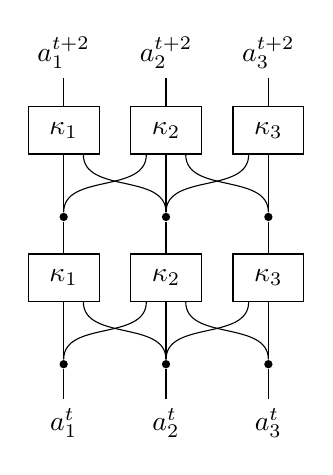
\begin{tikzpicture}[x=13mm, y=11mm]  % agents left to right, time bottom to top
    \foreach \i in {1,2,3} {
      \node[copy]   (c\i-0) at (\i,0.4) {};
      \node[kernel] (k\i-1) at (\i,1.4) {$\kappa_{\i}$};
      \node[copy]   (c\i-1) at (\i,2.1) {};
      \node[kernel] (k\i-2) at (\i,3.1) {$\kappa_{\i}$};
      \draw (\i,0) node[below] {$a_{\i}^{t}$} -- (c\i-0);
      \draw (k\i-1) -- (c\i-1);
      \draw (k\i-2) -- (\i,3.7) node[above] {$a_{\i}^{t+2}$};
    }
    % one pair j/i per edge j -> i of G; i/i = agent i's own last action
    \foreach \j/\i in {1/1, 2/2, 3/3, 1/2, 2/1, 2/3, 3/2} {
      \foreach \r/\s in {0/1, 1/2} {
        \draw (c\j-\r) to[out=90, in=-90] ($(k\i-\s.south)+({(\j-\i)*2.5mm},0)$);
      }
    }
  \end{tikzpicture}
  \caption{Composed prediction for a three-agent chain (with $k=1$) over two rounds. Time points up, and the dots are copy maps.}
  \label{fig:chain}
\end{wrapfigure}

The game we shall consider involves a repeated procurement auction with firms represented by agents.
An agent may either bid high or low, and they have a cheap-talk vocabulary consisting of three signals: ``I'll bid high'', ``I'll bid low'', and silence.
Each of our $n$ agents sits on a directed graph $G$; we read undirected graphs as directed ones by considering their edges bidirectional.
In round $t \in \{1, \ldots, T\}$, what agent $i$ sees is given in Table~\ref{tab:ladder}; it then emits its own action and, on the cheap-talk step, a signal; in the first round, agents can only see the prompt.
Every agent acts at once with the information from round $t-1$.

The payoff rule, described below, is told to agents in the prompt.
Agents are able to see their own last action as well as last round's payoff.
However, we do not provide them with a running total: when the full history is not shared with agents, a running total would bring long memory into the last-$k$ prompts of the calibration arm, and when it is, a running total may cause agents to weigh old rounds more heavily.
We do not disclose the number of rounds $T$ to agents, since disclosure would likely alter their behaviour in a way unrelated to communication or memory.

Our payoff $u_i \colon A \times F_i \to \mathbb{R}$, with $A = \{\mathrm{H}, \mathrm{L}\}$ (high or low) and $F_i = \{0, 1/d_i, \ldots, 1\}$, is given by $u_i(\mathrm{H}, f) = \uHL + f(\uHH - \uHL)$ and $u_i(\mathrm{L}, f) = \uLL + f(\uLH - \uLL)$; here, $d_i$ is the in-degree, and $f$ is the fraction of in-neighbours who bid high.
The parameters $\uLH, \uHH, \uLL, \uHL \in \mathbb{R}$ are values from an agent's bid (first subscript) and all of its neighbours' bids (second subscript).
Then, by imposing the ordering $\uLH > \uHH > \uLL > \uHL$ and $2\uHH > \uLH + \uHL$, we give our game the structure of the prisoner's dilemma.
Note that we do not assume our agents to optimize their payoff, and no result of ours depends on the payoffs.
Also, the payoff is not a function of signals, which thus have no cost to the agents.

We will currently take $(\uLH, \uHH, \uLL, \uHL) = (12, 10, 4, 0)$.
These values are subject to change.

% Information ladder: the "audit model sees" column defines q. Refer to steps by
% name; labelled actions (step 2) is parked.
\begin{table}[ht]
  \centering\small
  \begin{tabular}{@{}l p{0.3\textwidth} p{0.27\textwidth} l@{}}
    \toprule
    Step & Agents see & Audit model sees & Status \\
    \midrule
    Counts & How many neighbours took each action & The same & Core (control) \\
    Labelled actions & Each neighbour's action, by name & Counts & Parked \\
    Cheap talk & Action counts plus counts of each signal & Action counts only & Core (key step) \\
    Free text & Neighbours' messages & Messages sorted into a few categories & Conditional extra \\
    \bottomrule
  \end{tabular}
  \caption{Information ladder}
  \label{tab:ladder}
\end{table}

\begin{definition}[Swarm]\label{def:swarm}
    The set of possible records $R_i$ for agent $i$ contains all the information for agent $i$ over one round.
    A record $r^s_i \in R_i$, which is the information regarding agent $i$ that occurred in round $s$, holds, for round $s$, the agent's own action $a^s_i \in A$, its own signal $\sigma^s_i \in \Sigma$ on the cheap-talk step only, and its in-neighbours' counts at round $s$ described in Table~\ref{tab:ladder}.
    We denote by $H^t_i$ the set of all histories of agent $i$ at round $t$, which are each $(t-1)$-tuples $h^t_i = (r^1_i, \ldots, r^{t-1}_i) \in R^{\times(t-1)}_i$.
    As each component of a record comes from a finite set, $R_i$ is finite, and thus $H^t_i$ is finite, so every kernel below is a morphism of $\FinStoch$.
    We define $H_i = \bigsqcup_{t=1}^{T} H_i^t$ to be the set of histories of every length of agent $i$ across all rounds.
    
    We denote the kernel for the set of histories $H_i$ by $K_i \colon H_i \to O$, where the output set $O = A$ on the counts step and $O = A \times \Sigma$ on the cheap-talk step.
    The kernel assigns to each history in $H_i$ the probability distribution on $O$; given that each agent has the same model and prompt template, $K_i$ depends on $i$ only through $d_i$.
    It is the model's distribution over its output, given the prompt built from $h$, at temperature 1.
    A record for round $s$ is computed via $r^s_i = \rho_i(o^s)$, where $o^s \in O^n$ is the output of all agents in round $s$, and $\rho_i \colon O^n \to R_i$ keeps agent $i$'s output and counts its in-neighbours' outputs.

    We assume independent sampling, so $\mathbb{P}(o^t \mid o^1, \ldots, o^{t-1}) = \prod_i K_i(o^t_i \mid h^t_i)$, where $o^t_i$ is agent $i$'s output in round $t$, and $h^t_i = (\rho_i(o^1), \ldots, \rho_i(o^{t-1}))$.
    Then, multiplying over rounds gives us $\mathbb{P}(o^1, \ldots, o^T) = \prod_{t=1}^T \prod_i K_i(o^t_i \mid h^t_i)$, a distribution on $(O^n)^{\times T}$.
    For round 1, we have $h^1_i = ()$ from its definition, which matches the formula.
    Let $\mathrm{pr} \colon O \to A$ keep the action, so it is the identity on the counts step and drops the signal on the cheap-talk step.
    Thus, $a^t = (\mathrm{pr}(o^t_1), \ldots, \mathrm{pr}(o^t_n)) \in A^n$.
    The whole trajectory is $a_{1:T} = (a^1, \ldots, a^T)$.
    Finally, we denote the law of $a_{1:T}$ by $\mathcal{L}_{\text{swarm}}(a_{1:T})$.
\end{definition}
\begin{definition}[Audit and Prediction]\label{def:audit}    
    Let $q \colon R_i \to \overbar{R_i}$ keep agent $i$'s action and action counts, and drop its own signal and signal counts; here, $\overbar{R_i}$ is the image, the third column of Table~\ref{tab:ladder}.
    On a history $h$, we have $q(h) = (q(r^1), \ldots, q(r^{t-1}))$.
    Note that on outputs, we write $q$ for $\mathrm{pr}$ from Definition~\ref{def:swarm}.
    Let $\pi_k \colon q(H_i) \to S_i$ keep the last $k$ entries of a coarse history, where the coarse states $S_i$ are the tuples of $\overbar{R_i}$ of length at most $k$.
    Round 1 has the empty tuple as its coarse state; for rounds with fewer than $k$ earlier rounds, $\pi_k$ keeps all entries.
    
    We define $\ptest$ to be a distribution on $H_i$ so that every length $0, \ldots, T-1$ has positive probability, and we denote $\ptest(i, t)$ to be $\ptest$ conditioned on $H^t_i$.
    Let $\kappa_i \colon S_i \to A$ be the conditional expectation:
    \begin{equation}
        \kappa_i(\cdot \mid s) = \mathbb{E}_{h \sim \ptest}[\mathrm{pr}_* K_i(\cdot \mid h) \mid \pi_k(q(h)) = s].
    \end{equation}
    Note that this is only defined where $\ptest$ gives the state $s$ a positive probability; $\ptest$ gives every coarse state a positive probability.
    We define $\overbar{\rho_i} \colon A^n \to \overbar{R_i}$ to take agent $i$'s action and count its in-neighbours' actions.
    We have $q \circ \rho_i = \overbar{\rho_i} \circ \mathrm{pr}^n$, as counting actions only requires actions.

    Also, we define a composed chain, which is an order-$k$ Markov chain on $A^n$, given by $\mathbb{P}_{\text{model}}(a^t \mid \text{earlier profiles}) = \prod_i \kappa_i(a^t_i \mid \pi_k(\overbar{\rho_i}(a^1), \ldots, \overbar{\rho_i}(a^{t-1})))$.
    Note that our composite is, in effect, a dynamic Bayesian network.
    Finally, we denote the law of the chain's trajectory by $\mathcal{L}_{\text{model}}(a_{1:T})$.
\end{definition}

% One or two lines: the two sources of mismatch (memory beyond k rounds, what q
% drops). The calibration arm removes the first and the counts step the second,
% which is why H1 should be exact. A plain paragraph here also gives the
% wrapfigure above some text to wrap around.
One source of mismatch is memory beyond $k$ rounds, though the calibration arm only shows the last $k$ rounds, thus removing this source.
Another is that $q$ drops signals on the cheap-talk step.
Thus, the prediction should be exact only on the counts step of the calibration arm.
\section{Results}
% Budget: about half a page. Uses only Definitions 1 and 2 from Section 2.

\begin{definition}[Defect]
    Given a distribution $p$ on $H_i$, we define the defect $\varepsilon_i(p)$ to be given by
    \begin{equation}
        \varepsilon_i(p) \;=\; \mathbb{E}_{h \sim p}\; d_{\mathrm{TV}}\!\Big( q_{*}K_i(\,\cdot \mid h),\; \kappa_i\big(\,\cdot \mid \pi_k(q(h))\big) \Big),
    \end{equation}
    which is well-defined as $\ptest$ gives every coarse state a positive probability, so $\kappa_i$ is defined at $\pi_k(q(h))$.
    Let $\pswarm(i, t)$ be the law of $h^t_i = (\rho_i(o^1), \ldots, \rho_i(o^{t-1}))$ using the swarm process of Definition~\ref{def:swarm}; this is a distribution on $H^t_i$.
\end{definition}

\begin{theorem}[TV Bound]\label{thm:TV_bound}
    Given the assumptions found in Definition~\ref{def:swarm} and Definition~\ref{def:audit}, we have the following inequality.
    \begin{equation}
        d_{\mathrm{TV}}\big(\mathcal{L}_{\text{swarm}}(a_{1:T}),\, \mathcal{L}_{\text{model}}(a_{1:T})\big) \;\le\; \sum_{t=1}^{T} \sum_{i=1}^{n} \varepsilon_i\big(p_{\text{swarm}}(i,t)\big)
    \end{equation}
    This bound holds for any statistic $f$ of the trajectory $a_{1:T}$.
\end{theorem}
% \begin{proof}[Proof Sketch]
%     % Hybrids H_j; consecutive hybrids differ in one round; data processing; sum over
%     % rounds; the same bound for the law of any statistic of the trajectory.
%     \placeholder{Proof sketch}
    
% \end{proof}

\begin{proposition}[Exact Transfer]\label{prop:transfer}
    Given that, for every agent $i$, we have $\varepsilon_i(\ptest) = 0$, and $\mathop{\mathrm{supp}} \pswarm(i, t) \subseteq \mathop{\mathrm{supp}} \ptest$ for all $t$, we have $\mathcal{L}_{\text{swarm}}(a_{1:T}) = \mathcal{L}_{\text{model}}(a_{1:T})$.
  % Cite Fritz (2020) for the almost-sure calculus (add to refs.bib); a direct
  % probabilistic proof also exists.
\end{proposition}

% \begin{corollary}[\placeholder{name}]
%   \label{cor:coverage}
%   \placeholder{Local coverage check: statement}
% \end{corollary}

% \begin{remark}
%   % Cite Mitrophanov (2005) (add to refs.bib).
%   \placeholder{Worst case vacuous at realistic sizes; mixing-time version}
% \end{remark}

\section{Experiment}
\label{sec:experiment}

% Budget: about half a page. The table takes ~8 lines, leaving 2-3 lines per part.
% This section turns the objects of Section 2 into procedures: p_test (unit tests),
% the swarm law (swarm runs), p_swarm(i,t) (replay), and L_model (statistics).

% Run matrix, from the hand-off. "Runs" is per cell, i.e. per (step, n, graph, k):
% this is what the hand-off's Modal cost estimate assumes (e.g. the core sweep:
% 600k calls x 650 tokens at 5,000 tokens/s = 21.7 GPU-hours). Say so in the caption.
% Caption, still to write: T = 20 rounds throughout; what one run is; that the
% conditional extras run only if Saturday is clean, in the order numbered.
% To save space, the three conditional rows can collapse into one line of the caption.
\begin{table}[ht]
  \centering\footnotesize
  \setlength{\tabcolsep}{4pt}
  \begin{tabular}{@{}p{0.15\textwidth}llllll@{}}
    \toprule
    Arm & Steps & $n$ & Graphs & $k$ & Runs & Status \\
    \midrule
    Calibration (last $k$ rounds) & Counts, cheap talk & 4          & Chain, star, fully connected & 1, 2 & 100          & Committed \\
    Core (full history)           & Counts, cheap talk & 10, 20, 40 & Chain, star, fully connected & 1    & 100, 100, 50 & Committed \\
    Scale                         & Counts, cheap talk & 100        & Cycle, random 4-regular      & 1    & 50           & Committed \\
    \midrule
    Free text                     & Free text          & 10, 20, 40 & Cycle, random 4-regular      & 1    & 50           & Conditional 1 \\
    Second 7B family              & Cheap talk         & 10, 20, 40 & Chain, star, fully connected & 1    & 100, 100, 50 & Conditional 2 \\
    $\sim$70B model               & Counts, cheap talk & 10         & Chain, star, fully connected & 1    & 50           & Conditional 3 \\
    \bottomrule
  \end{tabular}
  \caption{Run matrix: $T = 20$ rounds; one round follows Table~\ref{tab:ladder}; estimated time to run is 45 GPU hours; conditional extras run if Saturday is clean, in given order}
  \label{tab:runs}
\end{table}

% UNIT-TEST PROTOCOL (how p_test is built; no swarm data is used here: say so).
%  - Test per in-degree class, not per agent: K_i depends on i only through d_i, so
%    one set of tests per distinct d_i (chain: 1, 2; star: 1, n-1; fully connected:
%    n-1; cycle: 2; random 4-regular: 4). This is why unit tests are affordable.
%  - For each coarse state s, ~20 synthetic histories h with pi_k(q(h)) = s.
%    Lengths uniform over the lengths that can produce s: the empty state () only
%    from length 0, every other state needs length >= 1. Make this agree with the
%    "uniform on {0, ..., T-1}" in Definition 2.
%  - Earlier rounds random: actions, counts, and signals on the cheap-talk step;
%    each round's payoff computed from them, so unit-test prompts have exactly the
%    same format as swarm prompts.
%  - Exact probabilities: action token before signal in the output format, so
%    pr_*K_i is the first token's probability from one forward pass. State what
%    happens to mass on invalid tokens (e.g. renormalise over H and L).
%  - kappa_i(. | s) = average over the histories for s; eps_i(p_test(i,t)) = mean
%    TV distance over histories of length t-1.
We test per in-degree class instead of per agent.
As $K_i$ depends on $i$ only through $d_i$, we have one set of tests per distinct $d_i$.
This also results in unit tests being affordable.
For each coarse state $s$, we have about 20 synthetic histories $h$ with $\pi_k(q(h)) = s$.
History lengths are uniform over the lengths that can produce $s$.
The empty state $()$ takes from length $0$, and every other state needs length at least one.
Each round's payoff is computed from that round's own action and the neighbour action counts, so the unit-test prompts have the same format as the swarm prompts.
The action token is before the signal in the output format, so $\mathrm{pr}_* K_i$ is the first token's probability from one forward pass.
For invalid tokens, we renormalize over $\mathrm{H}$ and $\mathrm{L}$.
The average over the histories for $s$ is given by $\kappa_i(\cdot \mid s)$, and the mean total-variation distance over histories of length $t-1$ is given by $\varepsilon_i(\ptest(i,t))$.


% SWARM RUNS (the swarm law of Definition 1).
%  - Temperature 1; actions and signals sampled each round; all agents' calls go to
%    the server as one batch per round (the synchronous update).
%  - Record the full outputs o^t, not just actions, so every history can be rebuilt
%    through rho_i; replay depends on this.
%  - Prompt conditions from Section 2 (point back, don't repeat): payoff shown, no
%    running total, T undisclosed, round 1 is the prompt alone, calibration prompts
%    cut to the last k rounds.
We choose a temperature of one, our actions and signals are sampled each round, and all agents' calls go to the server as a single batch per round.
We record the full outputs $o^t$, so every history can be obtained via $\rho_i$; this is required for replay.
Prompt conditions may be found in Section~\ref{sec:set-up}.

% REPLAY (how p_swarm(i,t) is estimated).
%  - ~5,000 recorded histories per (size, topology, step), each fed to a single
%    agent; exact probabilities; TV distance from kappa_i.
%  - Stratify the sample by round, so eps_i(p_swarm(i,t)) exists for every t:
%    Theorem 1 sums over t, and H2 compares round by round.
%  - Swarm data only scores the model and never fits it: say so (a reviewer will
%    check this; it is in the hand-off's risk table).
Our sample size is approximately 5000 recorded histories per size, topology, and step; they are each fed into a single agent.
We have exact probabilities, and the total-variation distance is obtained from $\kappa_i$.
We stratify the sample by round, so that $\varepsilon_i(\pswarm(i,t))$ exists for every $t$.
Theorem~\ref{thm:TV_bound} sums over $t$, and H2 compares each round.
The swarm data only scores the model; it does not fit the model.

% STATISTICS AND DELTA (L_model against the swarm).
%  - Statistics: fraction bidding high per round; time to consensus; final split.
%    Define consensus precisely (e.g. all agents take the same action for m
%    consecutive rounds), or time to consensus cannot be reproduced.
%  - Model side: Monte Carlo of the composed chain, with many more runs than the
%    swarm (it is cheap); exact for n = 4.
%  - Delta: TV distance between swarm and model distributions of each statistic;
%    bootstrap 95% intervals across runs. Bin statistics with many values: TV
%    between empirical distributions is biased upwards with many bins.
%  - Plot Delta against T with two curves: Theorem 1's bound with eps_i(p_swarm),
%    and the same sum with eps_i(p_test). Label the second a prediction, not a
%    bound: the theorem needs p_swarm.
%  - Short horizon: T = 5, from the first five rounds of each run (one clause).
Note that total variation, which is bounded by Theorem~\ref{thm:TV_bound}, between the two laws of a statistic, is a lower bound on the true trajectory distance (which is at most the bound), so we may use statistics to test our theorem.
We define $X_t = \tfrac{1}{n} \sum_i \mathbf{1}[a^t_i = \mathrm{H}]$, which gives one $\Delta_t$ per round; this is what the $\Delta$ versus $T$ plot needs.
The first round from which all agents take the same action for 3 consecutive rounds is denoted by $\tau$.
If we have no consensus, then we write $\tau = \infty$.
The final split is the average of $X_t$ over the last 5 rounds.

We have a Monte Carlo simulation of the composed chain, where each step only looks up $\kappa_i$, so $10^4$--$10^5$ runs are cheap, and the model's sampling noise becomes negligible.
For $n=4$, we may compute it exactly.
We estimate total variation from 100 samples, with the estimated total variation being biased upwards.
With $n=40$, $X_t$ takes 41 values, and two samples drawn from the same law can still give a total variation of $0.2$--$0.3$.
We thus bin $X_t$ into five bins of width $0.2$.
We measure the noise floor by taking two samples of the swarm's size from the model, compute the total variation between them, and plot it as a band.
Also, for a statistic with values in $[0, 1]$, $\lvert \mathbb{E}_{\text{swarm}} X_t - \mathbb{E}_{\text{model}} X_t \rvert \leq \Delta_t$, where we are considering unbinned $\Delta_t$, so we report the difference of means next to the binned total variation.
We bootstrap 95\% intervals across runs, resampling whole runs with replacement and recomputing $\Delta$.

Our plot of $\Delta$ against $T$ has two curves.
One is Theorem~\ref{thm:TV_bound}'s bound $B(t) = \sum_{s \leq t} \sum_i \varepsilon_i(\pswarm(i, s))$, and the other is the same sum with $\varepsilon_i(\ptest(i, s))$, which is a test-only prediction.

% BASELINES.
%  - Order-0 audit: kappa_i^0 = agent i's action distribution under p_test,
%    ignoring its coarse state; the composed chain then has independent agents.
%    Expected to fail, as in Ashery et al. (add to refs.bib).
%  - Order-1 audit: the method.
%  - Markov chain fitted to swarm data: the upper benchmark, as in Hirota et al.
%    (add to refs.bib). Say it is not an audit, since it uses swarm data. Fit on
%    half the runs and evaluate on the other half, so it cannot win by memorising.
% \placeholder{Baselines}

% The Friday pilot belongs with Section 6's milestones, not here.

\section{Hypotheses}

% Budget: about a quarter page. For each: the claim and what would falsify it.
\begin{itemize}
  \item[H1] We claim that on the counts step of the calibration arm, the prediction matches the swarm. This is tested by checking that $\Delta_t$ lies within the noise-floor band at every round and that $\varepsilon_i(\pswarm) = 0$ up to tolerance. It is falsified if these checks are negative, which would mean that there is a bug that must be fixed first.
  \item[H2] We claim that agents meet different situations in the swarm than in their tests, so $\varepsilon_i(\pswarm(i, t)) > \varepsilon_i(\ptest(i, t))$; the shift is larger on the cheap-talk step than on the counts step. This is measured by taking the difference of the two values averaged over agents and over rounds 2 to $T$. It is falsified if the interval for the shift includes zero, or if the cheap-talk shift is not larger than the counts shift.
  \item[H3] We claim that $\Delta_t$ levels off instead of growing linearly. This is measured via the slope of $\Delta_t$ over rounds 11 to 20 against the slope of the uncapped $B(t)$ over those rounds. It is falsified if the interval for $\Delta_t$'s slope reaches $B$'s slope. We only count where the fraction of runs already at consensus stays below a half.
  \item[H4] We claim that the order-0 audit fails where the order-1 audit holds. This is measured by $\Delta_t$ for order-0 against order-1 on the counts step of the core arm. It is falsified if order-0's $\Delta$ falls within order-1's interval. Note that the order-1 $\Delta$ should lie between order-0 and the chain fitted to swarm data.
  \item[H5] We observe whether $\Delta$ grows with $n$ as fast as the bound does, and whether the bound grows linearly in $n$. This is measured by the ratio $\Delta(n = 20) / \Delta(n = 10)$ against $B(20) / B(10)$ at round $T$ for each graph. Note that a ratio close to the bound's means that the bound is tight in $n$, and a smaller ratio means the gap grows more slowly than the bound. Our observation of effects across graphs with different topologies is exploratory.
\end{itemize}
% Commit in advance to reporting H2, H3 and H5 whichever way they come out.
We report H2, H3, and H5 in whatever order they come out.
% H1 is a gate, and H4 reproduces what is already known.

\section{Acknowledgement}

The prose in this set-up paper, up to grammatical and technical corrections, is entirely mine.
However, the paper was written with significant AI-assistance; large portions of the prose were written after conversations with AI.
Figure~\ref{fig:chain}, and the two tables present in this paper, as well as a lot of the technical \LaTeX{} code were created and written by AI.
This is largely representative of the time limit to write this paper imposed by the hackathon's start and end date.

\bibliographystyle{plainnat}
\bibliography{refs}
\end{document}
